\chapter{Die Domäne "`Internet of Things"'} \label{chap:DomainIot}
In diesem Kapitel wird die Domäne "`Internet of Things"' näher beschrieben und deren Auswirkungen auf die Softwareentwicklung aufgezeigt.



\section{Ziel}
Das primäre Ziel des \gls{acr:IOT} ist die Vernetzung von Dingen aus der realen Welt mit dem Internet und anderen Dingen. Die Dinge sollen intelligent und autonom mit anderen bekannten und unbekannten, Geräten und Anwendungen kommunizieren können um so ihre Fähigkeiten zu erweitern und einen Mehrwert für den Anwender zu schaffen. 



\section{Anwendungsbereich}
Das \gls{acr:IOT} kann grundsätzlich überall eingesetzt werden. Sei es in der Landwirtschaft, in der Pflege, in der Medizin oder in der Industrie. Das \gls{acr:IOT} ist mehr ein Konzept, beziehungsweise eine Architektur, als ein konkretes Produkt. Es kann als Querschnittsdomäne über alle anderen Domänen angesehen werden. Dadurch lässt es sich auf die jeweiligen Bedürfnisse der verschiedenen Problembereiche individuell anpassen. Neben der Anwendung im geschäftlichen Umfeld, findet das \gls{acr:IOT} auch im privaten Umfeld Anwendung. Dabei ist das primäre Ziel die Heimautomation, das heisst die intelligente Vernetzung verschiedener Geräte und Gegenstände im Haushalt.

Nachfolgend werden einige weitere Beispiele für die konkrete Anwendungen des \gls{acr:IOT} aufgelistet.


\begin{itemize}
\item Überwachung von Pflegepatienten (Notruf, Unfälle, Stürze)
\item Hausautomation (Schutz vor Einbrüchen, Energieoptimierung, Komfort)
\item Überwachung von Herstellungs- und Fertigungsprozessen
\item Überwachung von Gefahrensituationen in der Natur (zum Beispiel Waldbrände, Erdbeben, Felsstürze)
\end{itemize}

Auch im Bereich Big Data stellt \gls{acr:IOT} ein weiterer Meilenstein dar. Durch die Vernetzung von Millionen von Geräten können riesige Datenmengen gesammelt, analysiert und ausgewertet werden.


\section{Subdomänen und Verwandte Domänen}
Das \gls{acr:IOT} ist eine riesige Domäne mit vielen verschiedenen Anwendungsmöglichkeiten und somit auch vielen Subdomänen. Nachfolgend werden einige verwandte Domänen und Subdomänen aufgelistet und zwei spezifisch erläutert.

\begin{itemize}
\item Intelligente Städte ("`Smart Cities"')
\item Intelligentes Umweltmanagement ("`Smart Environment"')
\item Intelligentes Wassermanagement ("`Smart Water"')
\item Intelligente Messeinrichtungen ("`Smart Measuring"')
\item Sicherheit und Notfall ("`Security and Emergency"')
\item Logistik im Einzelhandel ("`Retail Logistics"')
\item Überwachung in der Industrie ("`Industrial Control"')
\item Intelligente Landwirtschaft ("`Smart Agriculture"')
\item Intelligente Massentierhaltung ("`Smart Animal Farming"')
\item Haushaltsautomatisierung ("`Domotics and Homeautomation"')
\item e-Health
\end{itemize}


\subsection{Wireless Sensor Network}
\gls{acr:WSN} sind Netzwerke von vielen verteilten Sensoren, welche gewisse physikalische Zustände oder Zustände in ihrer Umgebung und Umwelt überwachen. Die Forschung im Bezug auf \gls{acr:WSN}'s begann bereits in den 1980er und etablierte sich nach der Jahrtausendwende nach und nach in der Industrie. \gls{acr:WSN}'s entwickelten sich lange unabhängig vom \gls{acr:IOT}. Der Begriff \gls{acr:IOT} wurde zum ersten Mal um das Jahr 1999 erwähnt und tauchte in den darauffolgenden Jahren immer wieder auf. Heute kann gesagt werden, dass die beiden Bereiche immer mehr und mehr verschmelzen und die \gls{acr:WSN}'s als Teilbereich des \gls{acr:IOT} angesehen werden können. \gls{acr:WSN} kommen häufig in den Domänen Industrial Control, Smart Cities, Smart Environment und Smart Measuring zum Einsatz.


Ein \gls{acr:WSN}-Node ist ein billig produzierbares Gerät, welches nur sehr wenig Strom benötigt. Idealerweise wird dieses über eine Batterie oder eine autonome Energiequelle (zum Beispiel ein Solar-Panel) betrieben. \gls{acr:WSN}-Nodes besitzen meistens nur eine einzelne Funktion und sind in der Regel mit einem \gls{acr:WSN}-Edge-Node, beziehungsweise einem Gateway, verbunden.

Ein \gls{acr:WSN}-Edge-Nodes verbindet mehrere \gls{acr:WSN}-Nodes mit einem Netzwerk oder dem Internet. Dieser Edge-Node nimmt die Funktion eines Gateways wahr und kommuniziert mit einem Back-End System. Der Benutzer greift entweder über das Back-End System oder das Gateway auf die gesammelten Daten zu.

\begin{figure}[!h]
  \centering
  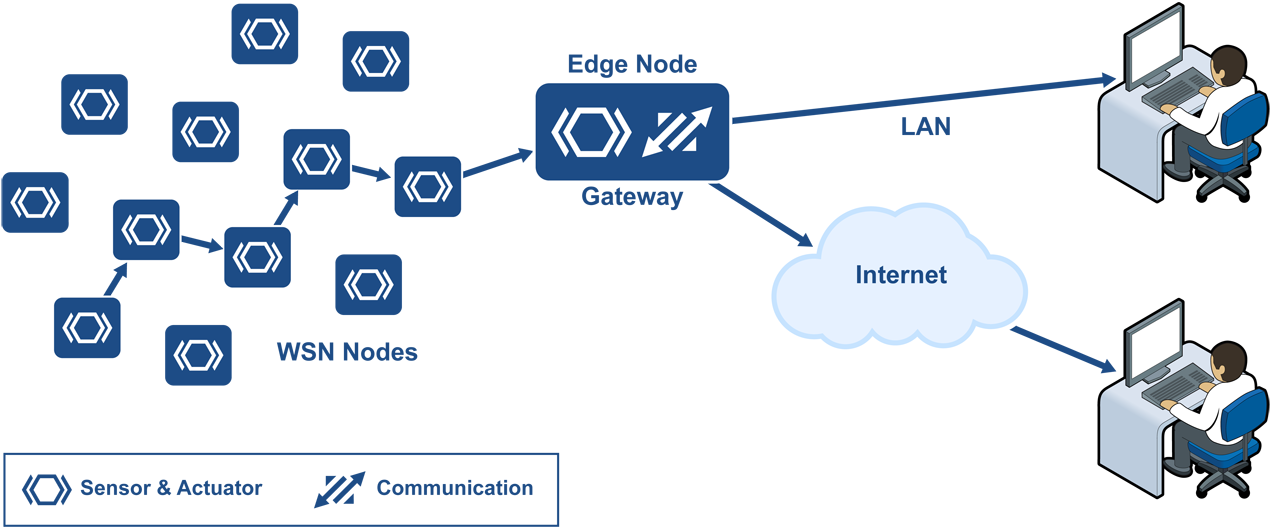
\includegraphics[width=10cm]{./images/wireless-sensor-network}
  \captionsource{Schematische Darstellung eines \gls{acr:WSN}}{\url{http://micrium.com/iot/devices/}}
  % Quelle: http://micrium.com/wp-content/uploads/2014/03/wireless-sensor-network.png
\end{figure}


Als Kommunikationstechnologie kommt entweder Wi-Fi oder eine drahtlose Low-Power-Lösung zum Einsatz. Der Vorteil von Wi-Fi besteht in seiner hohen Akzeptanz, Kompatibilität und Verbreitungsgrad. Dem Gegenüber steht der hohe Energieverbrauch von Wi-Fi. Inzwischen gibt es eine breite Palette an Low-Power-Lösungen welche für den Einsatz auf solchen Geräten optimiert sind. Sie sind energieeffizient, für lange Laufzeiten ausgelegt und verfügen meistens über die Fähigkeit ein Mesh-Network zu bilden. In einem Mesh-Network (Maschen-Netzwerk) müssen nicht alle Geräte eine direkte Verbindung mit dem Gateway aufweisen. Es ist ausreichend, wenn es in der Nähe eines Nodes einen anderen Node gibt, der entweder direkt oder indirekt mit einem Gateway verbunden ist. In der nachfolgenden Abbildung wird ein solches Mesh-Network schematisch dargestellt.



\begin{figure}[!h]
  \centering
  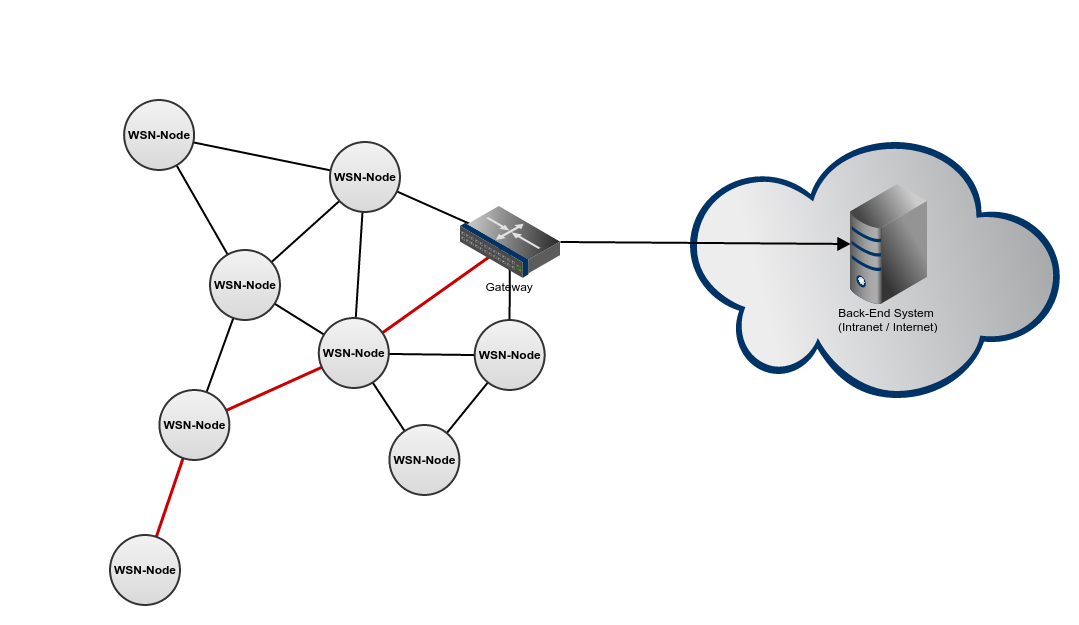
\includegraphics[width=10cm]{./images/Mesh-Network}
  \caption{Schematische Darstellung eines Mesh-Networks}
  % Quelle: http://micrium.com/wp-content/uploads/2014/03/wireless-sensor-network.png
\end{figure}


Der IEE 802.15.4 Standard wurde zum Beispiel speziell für den Einsatz in Low-Power-Systemen konzipiert. Die Standards, Protokolle und Frameworks welche im \gls{acr:IOT} Verwendung finden werden im Kapitel \ref{sec:SWDesignConstruction} \nameref{sec:SWDesignConstruction} erläutert.


\subsection{Heimautomation}
Bei der Heimautomation steht die Vernetzung und intelligente Kommunikation der Endgeräte untereinander im Vordergrund. Dabei kommt ein bunter Mix an unterschiedlichen Geräten und Technologien zum Einsatz, was eine enorme Herausforderung für die autonome Kommunikation unter den Geräten darstellt. Mit dem Einsatz eines Homeautomation- oder Smart-Gateways können diese Herausforderungen reduziert werden. Diese Gateways unterstützen eine breite Palette an Übertragungs- und Kommunikationsprotokollen und sind so in der Lage zwischen den Geräten zu vermitteln und übersetzen.

\begin{figure}[!h]
  \centering
  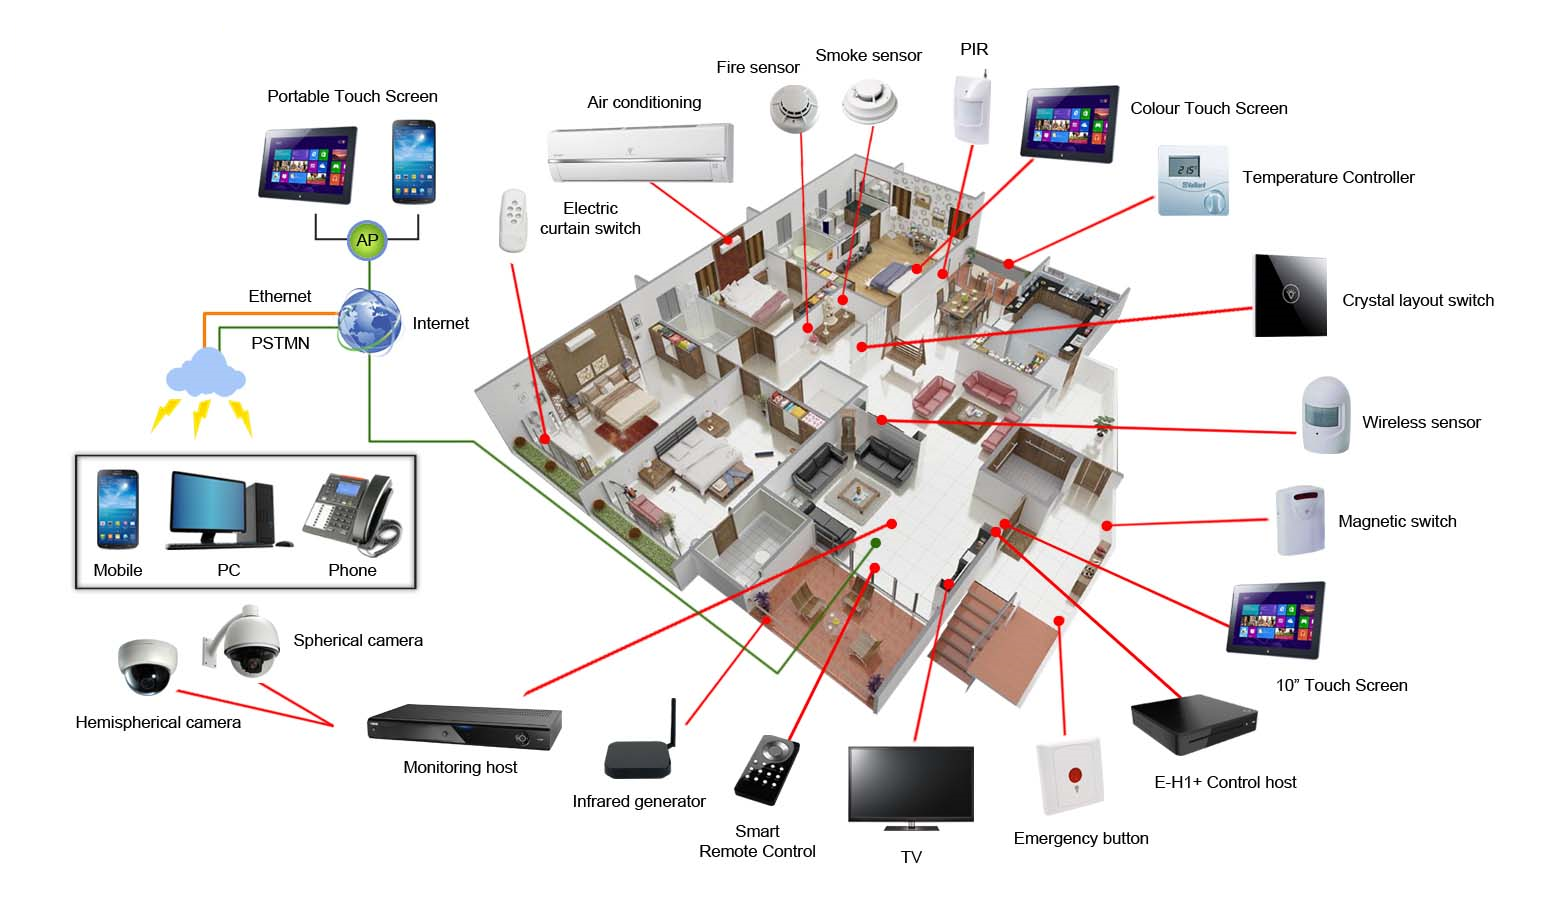
\includegraphics[width=14cm]{./images/smart_home_system}
  \captionsource{Szenario eines Heimautomatisierungs-Netzwerkes}{\url{http://www.witura.com/wifi-smart-home-management-system.html}}
  % Quelle: http://www.witura.com/images/smart_home_system_1.png
\end{figure}


\section{Architektur \& Aufbau}
Das \gls{acr:IOT} besteht vereinfacht dargestellt aus "`Things"', "`Gateways"' und "`Back-End Systems"', welche miteinander kommunizieren. In diesem Kapitel werden diese drei Elemente und deren Verbindungen untereinander beschrieben.

In der nachfolgenden Grafik wird der Kommunikationsweg innerhalb eines \gls{acr:WSN}'s aufgezeigt. Das "`Thing"' empfängt die Daten von einem Sensor, verarbeitet diese und benachrichtigt anschliessend über ein definiertes Protokoll das Gateway. Das Gateway empfängt die Daten von einem oder mehreren Sensoren, verarbeitet diese und benachrichtigt anschliessend das Back-End System. Die Benachrichtigung des Back-End Systemes erfolgt häufig über ein Standard Protokoll aus der Web-Domäne. Das Back-End System empfängt die Daten, verarbeitet diese und entscheidet, ob allenfalls weitere Schritte unternommen werden müssen. Zum Beispiel könnte er bei Überschreiten eines Grenzwertes den Benutzer via SMS informieren.

\begin{figure}[!h]
  \centering
  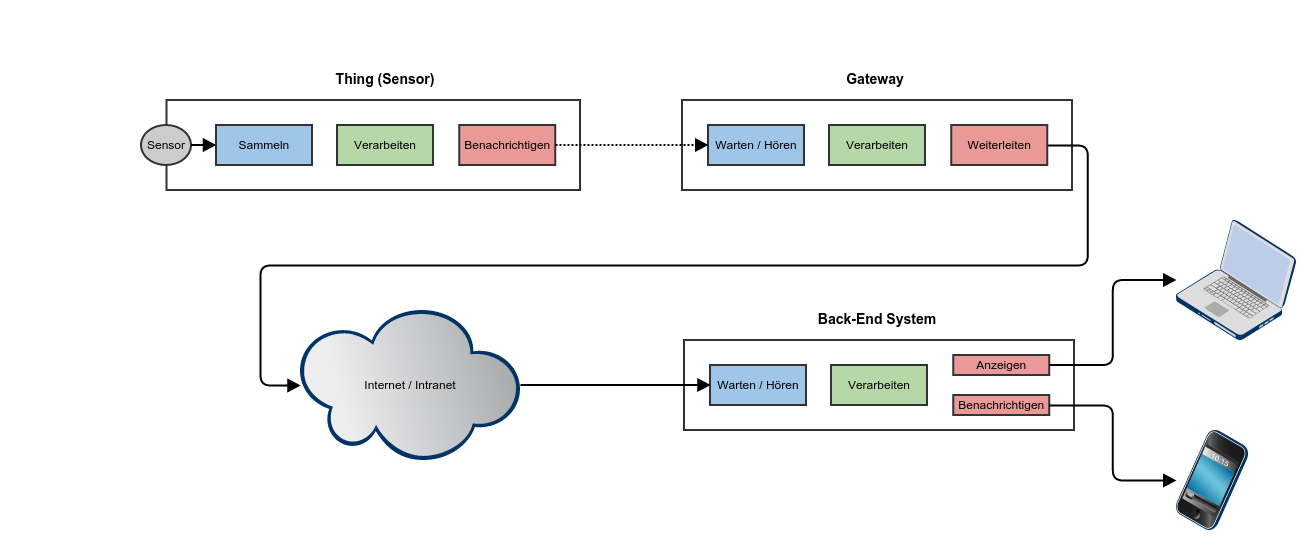
\includegraphics[width=16cm]{./images/Node-Gateway-BackEnd}
  \caption{Beispielhafter Aufbau eines Kommunikationsweges innerhalb eines \gls{acr:WSN}.}
\end{figure}

\subsection{Das "`Thing"'}
Die Definition eines "`Things"' (oder auch "`Smart Thing"'), beziehungsweise eines "`Dinges"', ist nicht ganz einfach. Grundsätzlich handelt es sich um einen physischen Gegenstand, ein "`Embedded Device"' (auch Embedded System genannt) welches gewisse Funktionalitäten anbietet. Dies können Sensoren oder auch Kontroll- oder Steuerungselemente sein. Handelt es sich bei diesem "`Ding"' um einen Alltagsgegenstand, wird dieser auch als "`Smart Object"' bezeichnet. Ein "`Embedded Device"' basiert auf einem Mikrocontroller, verfügt relativ gesehen nur über geringe Ressourcen (Prozessor, Arbeitsspeicher, Energie). Das "`Embedded Device"' verfügt über einen definierten Stack an Kommunikationsprotokollen, welche entweder direkt oder über ein Gateway mit einem Back-End System kommuniziert. 

Diese "`Dinge"' und "`Smart Objects"' sind nicht neu. Sie haben jedoch erst mit Aufkommen des \gls{acr:IOT} gelernt untereinander und mit dem Internet zu kommunizieren und autonom zu interagieren. Embedded Systems sind bereits heute überall gegenwärtig. Sei es in Autos, Wearables, Kühlschränken, Kaffeemschinen oder Smartphones.

Gemäss \cite{E:MachinaResearch:IoTWhitePaper} haben die "`Things"' und die \gls{acr:M2M}-Kommunikation folgende Phasen durchlaufen:

\begin{itemize} 
\item \textbf{Reactive information} \\Polling der Geräte zur Abfrage von Informationen.
\item \textbf{Proactive information} \\Geräte Kommunizieren die Informationen wenn dies notwendig ist.
\item \textbf{Remotely controllable} \\Geräte sind aus der Ferne steuerbar.
\item \textbf{Remotely serviceable} \\Geräte sind aus der Ferne wartbar.
\item \textbf{Intelligent processes} \\Geräte sind Teil von intelligenten Prozessen.
\item \textbf{Optimised propositions} \\Gesammelte Informationen der Geräte können für die Entwicklung von neuen Produkten verwendet werden.
\item \textbf{New business models} \\Neue Möglichkeiten für Geschäftsmodelle.
\item \textbf{The Internet of Things} \\Teilung von Informationen mit Geräten von Dritt-Herstellern, um im gesamten einen Mehrwert zu generieren
\end{itemize}

\subsection{Gateway / Bridge}
Die Aufgabe eines Gateways, ab und zu auch als Bridge bezeichnet, ist es, "`Things"' mit einem Netzwerk zu verbinden. Oft sind "`Things"' nicht in der Lage sich direkt mit einem Netzwerk oder dem Internet zu verbinden. 85 \% aller "`Things"' sind heute nicht in der Lage direkt mit dem Internet zu kommunizieren \cite[S. 2]{E:Intel:WhitePaper:DevelopingSolutionsIoT}. In solchen Situationen wird ein Gateway eingesetzt, welches diese Lücke schliesst. Eine weitere Aufgabe eines Gateways kann die intelligente Filterung und Zusammenfassung von Daten sein, bevor diese an das Back-End System weitergeleitet werden. Dadurch wird verhindert, dass durch die gesammelten Datenmassen der "`Things"' quasi ein \gls{acr:DDOS}-Angriff auf das Back-End System erfolgt.


\subsection{Back-End Systeme}
Die Back-End Systeme stehen oft in einem Netzwerk oder in der Public-Cloud, wo diese entsprechend den Bedürfnissen skaliert werden können. Zum Einsatz kommen Systeme zur Analyse und Auswertung der gesammelten Informationen. Bei sehr grossen Datenmengen werden typischerweise Big-Data-Systeme eingesetzt. Je nach Anwendungsbereich können die gesammelten und ausgewerteten Daten über einen Computer, ein mobiles Gerät oder ein anderes System abgerufen und weiterverwendet werden. Handelt es sich um ein Automatisierungssystem ist zusätzlich noch eine Steuer-Komponente integriert, welche auf Basis von Regeln und Benutzereingaben die Steuerung der Geräte übernimmt.


\subsection{Das "`Web of Things"'}
Das "`Web of Things"' hat sich aus dem \gls{acr:IOT} entwickelt und ist ein Architekturansatz, welcher vorsieht alle \gls{acr:IOT}-Geräte in das bestehende Internet / Web einzubinden. Dazu sollen bereits für das Web etablierte Standards wie zum Beispiel HTTP, HTTPS, RSS oder REST zum Einsatz kommen. Auf jedem Gerät müsste ein minimaler Web-Server vorhanden sein, durch welchen die Integration in das Web erfolgt. Der Vorteil dieser Architektur liegt darin, dass alle bestehenden Möglichkeiten des Webs voll ausgenutzt werden können. Der grösste Nachteil ist, dass die heutigen Web-Protokoll nicht sehr sparsam mit Ressourcen (Hardware, Strom) umgehen.

\subsection{Referenz Modelle und Referenz Architekturen}
Zum heutigen Zeitpunkt gibt es  mehrere Ansätze ein Referenz Model und eine Referenz Architektur für das \gls{acr:IOT} zu schaffen.

Nachfolgend werden einige dieser Referenz Modelle und Architekturen aufgelistet, jedoch aufgrund von deren Umfang und Komplexität nicht im Detail erläutert.

\begin{itemize}
\item \textbf{IoT-A}\\
\url{http://www.iot-a.eu/}
\item \textbf{WSO2 - A Reference Architecture for the Internet of Things}\\
\url{http://wso2.com/whitepapers/a-reference-architecture-for-the-internet-of-things/}
\item \textbf{IoT@Work - Final Framework Architecture Speciffication}\\
\url{https://www.iot-at-work.eu/downloads.html}
\item \textbf{Internet of Things Architecture (u.a. Cisco, IBM, Intel)}\\
\url{https://www.iotwf.com/iotwf2014/breakout}
\end{itemize}


\section{Unterschied zum Konzept des klassischen Internet}
In der klassischen Auslegung des Internets stellen zentrale Server die Daten zur Verfügung, welche dann von Anwendern oder Bezügern abgerufen werden können. Die Datenhoheit liegt dabei bei diesen zentralen Servern. Kommuniziert wird entweder von Server zu Server oder von Anwender / Bezüger zu Server. Es war immer ein Server als intermediär notwendig. Das \gls{acr:IOT} bringt nun einen Paradigmenwechsel mit sich. Die Geräte in einem \gls{acr:IOT} sind in der Lage autonom miteinander zu kommunizieren und zu interagieren. 

Im klassischen Internet werden im Vergleich grosse Datenmenge pro Packet transportiert. Im \gls{acr:IOT} ist dies nicht mehr notwendig, da dort in der Regel nur kleine Datenmengen, jedoch in sehr grossen Stückzahlen, übermittelt werden müssen. Auch ist es nicht essentiell, dass alle Pakete beim Ziel ankommen, da der Wert eines einzelnen Datenpacketes	sehr gering ist.


Das \gls{acr:IP} und \gls{acr:TCPIP} sind auf stabile Netzwerke ausgelegt, in welchen grosse Datenmengen zuverlässig transportiert werden müssen. Die Anforderungen des \gls{acr:IOT} nach sich verändernden und dynamischen Netzwerken, sehr kleinen Datenmengen, vielen Requests und eingeschränkten Geräten werden durchdie heutigen Protokolle und Standards nicht optimal abgedeckt. Um den maximalen Nutzen zu erreichen werden neue, spezifische Protokolle und Standards benötigt



\section{Effekte \& Auswirkungen}
Durch den Einsatz eines \gls{acr:IOT} kann Mehrwert in verschiedensten Bereichen und Ebenen geschaffen werden. Das \gls{acr:IOT} wird zahlreiche neue Geschäftsmodelle und Produktpaletten hervorbringen, welche sowohl einen Mehrwert für den Hersteller, als auch für den Konsumenten generieren. Neben den positiven Effekten sind auch die negativen Effekte nicht zu vernachlässigen. Im Kapitel \ref{sec:DomainIoT:Challenges} \nameref{sec:DomainIoT:Challenges} werden die verschiedenen Herausforderungen erläutert, welche das \gls{acr:IOT} mit sich bringt. 



\section{Herausforderungen} \label{sec:DomainIoT:Challenges}
Im \gls{acr:IOT} gibt es viele Herausforderungen zu bewältigen. Die wichtigsten werden nachfolgend aufgelistet:

\begin{itemize}
\item Verfügbarkeit eines Internet-Zuganges am Einsatz- / Verwendungsort
\item Sicherheit und Datenschutz
\item Tiefe Kosten für Hard- und Software
\item Energieversorgung
\item Energieverbrauch
\item Skalierbarkeit
\item Fehlertoleranz
\item Akzeptanz
\item Robustheit (physisch und logisch)
\item Entdecken von Geräten und Services (Device Discovery)
\item Fernwartung von Geräten und Anwendungen
\end{itemize}

Einige dieser Herausforderungen haben grössere Auswirkungen auf die Software-Entwicklung im Bereich \gls{acr:IOT}. Ist in der normalen Softwareentwicklung eine Trennung der spezifischen Themen (Separation of Concerns) ohne weiteres möglich, ist dies im \gls{acr:IOT} nicht ohne weiteres der Fall. Für die Entwicklung eines "`Things"' sind Fähigkeiten aus den Bereichen "`Distributed Systems"', "`Embedded Systems"', "`Networking"', "`Operating Systems"' und "`Software Development"' erforderlich. Entweder muss ein Entwickler all diese Skills mitbringen oder die Architektur muss die Trennung / Abstraktion der verschiedenen Schwerpunkte erlauben, sodass diese vom jeweiligen Spezialisten implementiert werden können. Um diesem breiten Spektrum an notwendigen Fähigkeiten gerecht zu werden sind heutige allgemeine \gls{acr:DSL}'s nicht geeignet. Der Ansatz "`one size fits all"' ist hier nicht ideal. Eine \gls{acr:IOT} \gls{acr:DSL} sollte entsprechende Mittel zur Abstraktion und Trennung vorsehen, um eine effiziente Entwicklung zu ermöglichen. 

Weitere Herausforderungen sind die Heterogenität der Geräte, die Skalierbarkeit und die Implikationen im Bezug auf die rechtlichen Aspekte. Zu klären ist hier, wem die gesammelten Daten gehören (dem Betreiber des Gerätes? dem Betreiber des Back-End-Systemes, welches für die Analyse benötigt wird?) und wer für Aktionen verantwortlich ist, welche das Gerät selbstständig ausgeführt hat. 

Beispiel: Ein Kühlschrank bestellt bei einem Lebensmittelhändler eine grosse Menge an Milch nach, da gemäss den Berechnungen und Analysen des Systems der Milchvorrat zu niedrig ist. Der Besitzer benötigt diese Milch jedoch gar nicht. Da der Kühlschrank nicht haftbar ist, stellt sich nun die Frage nach einer haftbaren Person. Ist es der Besitzer? Die Herstellerfirma? Der Entwickler? Dieses Beispiel mag banal sein, aber in der Industrie oder in der Medizintechnik können kleine Berechnungsfehler oder Fehleinschätzungen massive Auswirkungen haben, was auch entsprechend hohe Kosten nach sich ziehen kann.



\section{Anforderungen an das Produkt und die Software}
Aufgrund der Besonderheiten der Domäne \gls{acr:IOT} ergeben sich auch einige spezifische Anforderungen an das Produkt und die verwendete Software. Das Gerät und die Software sollten für den sie bestimmten Zweck über ausreichend leistungsfähige Ressourcen verfügen und entsprechend skaliert werden können.  Zugleich muss mit den Ressourcen so schonend wie möglich umgegangen werden, um eine möglichst lange Laufzeit zu erreichen. "`Things"' verfügen meistens über eine mobile Energiequelle, wie zum Beispiel eine Batterie oder einen Akku, oder eine erneuerbare Energiequelle. Daneben spielt auch die Sicherheit und der Datenschutz eine grosse Rolle, da die Geräte nicht permanent überwacht werden können. Hinzu kommen auch regulatorische und rechtliche Aspekte, Herausforderungen und Anforderungen, welche es zu berücksichtigen gibt.

Aufgrund des grossen Anwendungsgebietes ist auch das Spektrum an Anforderungen entsprechend gross. Bei einem Kühlschrank, welcher Teil eines \gls{acr:IOT}'s oder Heimautomationsnetzwerkes ist, spielt die energieeffizienz oder grösse des Gerätes nicht zwingend eine grosse Rolle. Grund dafür ist, dass der Kühlschrank im Vergleich sehr viel Platz aufweist und an eine permanente Stromquelle angeschlossen ist.

Im Kapitel \ref{chap:sweInIot} \nameref{chap:sweInIot} werden die Unterschiede und speziellen Anforderungen an das Software Engineering in der Domäne "`Internet of Things"' im Vergleich zur "`Standard Domäne"' aufgezeigt.
